%
% newton.tex
%
% (c) 2020 Prof Dr Andreas Müller, Hochschule Rapperswil
%
\section{Newton-Verfahren
\label{buch:section:newtion}}
\rhead{Newton-Verfahren}
\index{Newton-Verfahren}%
Die bisher vorgestellten Verfahren zur Bestimmung einer Nullstelle
$x^*$ der Funktion $f$, $f(x^*)=0$ sind linear konvergent und damit
eher langsam.
\index{Nullstelle}%
Dafür war nicht mehr als Stetigkeit nötig, um Konvergenz des Verfahrens
sicherzustellen.

%
% Analytischer Ansatz
%
\subsection{Analytischer Ansatz für ein quadratisch konvergentes Verfahren
\label{buch:subsection:newton:analytisch}}
In Abschnitt~\ref{buch:subsection:linearekonvergenz} wurde dargestellt,
dass nach Möglichkeit quadratische Konvergenz angestrebt werden sollte.
\index{quadratische!Konvergenz}%
\index{Konvergenz!quadratisch}%
Quadratische Konvergenz könnte in einer Fixpunktiteration $x_{n+1}=g(x_n)$
erreicht werden, wenn die Ableitung $g'(x^*)=0$ ist.
\index{Fixpunkt}%

Je grösser $f(x_n)$ ist, desto weiter dürfte $x_n$ von der Nullstelle
entfernt sein.
Wir versuchen daher, die Approximation $x_{n+}$ proportional zum Wert von
$f(x_n)$ zu korrigieren mit Hilfe der Funktion
\[
x_{n+1} = g(x_n) = x_n - a(x_n)\cdot f(x_n).
\]
Die Funktion $a(x_n)$ muss noch bestimmt werden.
Sie soll so gewählt werden, dass die Konvergenz quadratisch wird, was
mit $g'(x^*)=0$ erreicht wird.

Die Ableitung von $g$ ist
\begin{align*}
g'(x)
&=
1-a'(x)f(x)-a(x)f'(x).
\intertext{An der Stelle $x^*$ gilt}
g'(x^*)
&=
1-a'(x^*)\underbrace{f(x^*)}_{\displaystyle=0} - a(x^*)f'(x^*) = 0
\\
\Leftrightarrow\qquad
1
&=
a(x^*) f'(x^*)
\qquad\Rightarrow\qquad
a(x)=\frac{1}{f'(x)}.
\end{align*}
Damit finden wir das im folgenden Satz beschriebene Verfahren mit
quadratischer Konvergenz.

\begin{satz}[Newton-Verfahren]
\index{Newton-Verfahren}%
\label{buch:satz:newton-verfahren}
Hat die differenzierbare Funktion $f$ eine Nullstelle $x^*$ und gilt
$f'(x^*)\ne 0$, dann konvergiert die Iterationsfolge
\begin{equation}
x_{n+1} = x_n - \frac{f(x_n)}{f'(x_n)} 
\label{buch:equation:newtoniteration}
\end{equation}
für Startwerte $x_0$ genügend nahe bei $x^*$ quadratisch gegen die
Nullstelle.
\end{satz}
\index{Startwert}%

Das Sekantenverfahren hat darunter gelitten, dass die Berechnung
der der nächsten Approximation mit Hilfe der Formel 
\eqref{buch:eqn:sekanten-iteration} von umso stärker Auslöschung
geplagt ist, je näher man bereits an der Lösung ist.
\index{Sekantenverfahren}%
Die Iterationsformel
\eqref{buch:equation:newtoniteration}
für die Newton-Iteration hat dieses Problem nicht.
In \eqref{buch:equation:newtoniteration} wird der aktuelle Wert $x_n$
um einen Korrekturbetrag korrigiert, der proportional zu $f(x_n)$
verkleinert wird.
Je genauer der Wert $x_n$ schon ist, desto kleiner wird auch die
Korrektur.

%
% Geometrische Interpretation
%
\subsection{Geometrische Interpretation des Newton-Verfahrens}
\begin{figure}
\centering
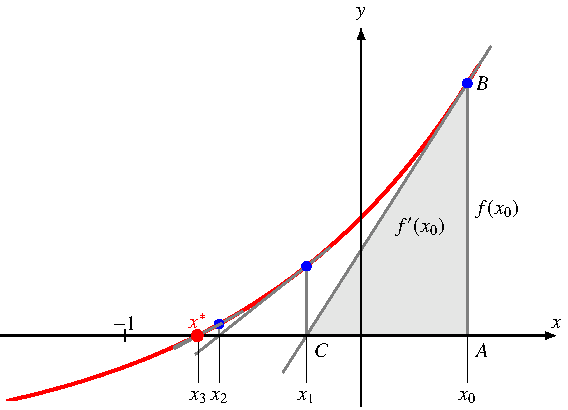
\includegraphics{chapters/20-gleichungen/figures/newton.pdf}
\caption{Graphische Interpretation des Newton-Verfahrens.
In jedem Iterationsschritt wird die bisherige Approximation $A$
mit Hilfe einer Tangente vom Funktionswert $B$ zum Punkt $C$
korrigiert, $\overline{AC}=f(x_0)/f'(x_0)$.
\label{buch:figure:newton}}
\end{figure}
Die Iterationsformel~\eqref{buch:equation:newtoniteration}
lässt sich sehr schön graphisch interpretieren.
In Abbildung~\ref{buch:figure:newton} wird die Nullstelle der
Funktion $f(x) = e^x-\frac12$ mit dem Newton-Verfahren bestimmt.
Im Iterationsschritt wird die Approximation $x_n$ korrigiert
nach der Formel
\[
x_{n+1}
=
x_n - \frac{f(x_n)}{f'(x_n)}
=
x_n - \frac{e^{x_n}-\frac12}{e^{x_n}}
=
x_n - \biggl(1 -\frac{e^{-x_n}}{2}\biggr)
\]
Die Korrektur für $n=0$ ist in Abbildung~\ref{buch:figure:newton}
als Grundseite des rechtwinkligen Dreiecks $ABC$ erkennbar.
Die Hypothenuse hat die Steigung $f'(x_0)$, daher ist
\index{Hypothenuse}%
\index{Dreieck}%
\[
\overline{AC}\cdot f'(x_0) = f(x_0)
\qquad\Rightarrow\qquad
\overline{AC} = \frac{f(x_0)}{f'(x_0)}.
\]
Die vom Newton-Verfahren berechnete Korrektur ist also die optimale
Korrektur, die sich aus Funktionswert und erster Ableitung
an der Stelle $x_n$ berechnen lässt.
\index{Ableitung}%

%
% Wurzeln
%
\subsection{Wurzeln}
Als Beispiel für die Anwendung des Newton-Verfahrens berechnen wir die
$k$-te Wurzel einer positiven reellen
Zahl $a$, wir lösen also die Gleichung
$x^k = a$.
\index{Wurzel}%
Dies ist gleichbedeutend damit, eine Nullstelle der Funktion
$f(x)=x^k-a$ zu bestimmen.
Die Ableitung von $f$ ist
$f'(x)=kx^{k-1}$, woraus wir die Iterationsformel des
Newton-Verfahrens ablesen können:
\[
x_{n+1} = x_n - \frac{f(x_n)}{f'(x_n)}=x_n - \frac{x_n^k-a}{kx_n^{k-1}}
=
\frac{1}{k}\biggl((k-1)x_n+\frac{a}{x_n^{k-1}}\biggr).
\]
Im Falle $n=2$ finden wir das bereits in 
Abschnitt~\ref{buch:subsection:linearekonvergenz}
untersuchte, quadratisch konvergente Verfahren zur Bestimmung
der Quadratwurzel wieder.
\index{Quadratwurzel}%
In Tabelle~\ref{buch:table:wurzel5newton} ist das Verfahren für
$a=10$, $k=5$ und $x_0=a$ gezeigt.
Quadratische Konvergenz stellt sich allerdings erst bei $x_{10}$ ein,
der Startwert $x_0$ ist zu weit von der Lösung entfernt.

\begin{table}
\centering
\renewcommand\arraystretch{1.15}
\begin{tabular}{|>{$}r<{$}|>{$}r<{$}|}
\hline
n& x_n\\
\hline
 0 & 10.00000000000000\\
 1 &  8.00020000000000\\
 2 &  6.40064823242493\\
 3 &  5.12171019598693\\
 4 &  4.10027465454472\\
 5 &  3.28729556684556\\
 6 &  2.64696320430731\\
 7 &  2.15831219143923\\
 8 &  \underline{1}.81881622015378\\
 9 &  \underline{1.}63781027109793\\
10 &  \underline{1.58}820394873794\\
11 &  \underline{1.5849}0696686523\\
12 &  \underline{1.584893192}70054\\
13 &  \underline{1.58489319246111}\\
\hline
\infty&\sqrt[5]{10}=1.58489319246111\\
\hline
\end{tabular}
\caption{Berechnung von $\sqrt[5]{10}$ mit dem Newton-Verfahren.
Der Startwert $x_0=10$ ist sehr weit von der Lösung entfernt, so dass es
einige Iterationen braucht, bis die Konvergenz quadratisch wird.
\label{buch:table:wurzel5newton}}
\end{table}

%
% Newton-Verfahren in R^n
%
\subsection{Newton-Verfahren in $\mathbb R^n$
\label{buch:section:newtoninRn}}
\index{Newton-Verfahren!in $\mathbb R^n$}%
In der bisher beschriebenen Form erlaubt das Newton-Verfahren, 
Nullstellen von rellwertigen Funktion zu finden.
Es eignet sich nicht, Vektorgleichungen zu lösen.
\index{Vektorgleichung}%

Sei daher im folgenden $f\colon \mathbb R^k \to \mathbb R^k$ eine
Vektorfunktion mit einer Nullstelle $x^*$, $f(x^*)=0$, die numerisch gefunden 
werden soll.
Wie in Abschnitt~\ref{buch:subsection:newton:analytisch} soll eine
Approximation $x_n$ für die Nullstelle $x^*$ proportional zur Grösse
von $f(x_n)$ korrigiert werden.
Eine skalare Funktion $a(x)$ wird aber im allgemeinen zu wenig
allgemein für eine performante Lösung des Problem sein, daher
wird für $A(x)$ eine matrixwertige Funktion mit Werten in
$\operatorname{GL}_k(\mathbb R)$ gewählt.
\index{Funktion!matrixwertig}%
\index{GLkR@$\operatorname{GL}_k(\mathbb R)$}%
Wir setzen also an
\[
x_{n+1} = g(x_n) = x_n - A(x_n) f(x_n)
\]
und versuchen wie früher $A(x)$ so zu wählen, dass die Ableitung von $g$
an der Stelle $x^*$ verschwindet.

Die Ableitung von $g(x)=x-A(x)f(x)$ ist
eine lineare Abbildung, die auf dem Vektor $h\in\mathbb R^k$ den Wert
\begin{align*}
Dg(x) \cdot h
&=
h - (DA(x)\cdot h) f(x) - A(x) Df(x)\cdot h
\end{align*}
hat.
An der Stelle $x=x^*$ verschwindet der mittlere Term wegen $f(x^*)=0$, so
dass als Gleichung für $A(x)$
\[
0=h-A(x) Df(x) \cdot h
\qquad\Rightarrow\qquad
h = A(x) Df(x) \cdot h\qquad \forall h\in\mathbb R^n
\]
übrigbleibt.
Dies ist nur möglich, wenn $A(x)$ die inverse Matrix von $Df(x)$ ist,
was den folgenden Satz motiviert.

\begin{satz}[Newton-Verfahren für Vektorgleichungen]
\label{buch:satz:newtonVektorgleichungen}
\index{Newton-Verfahren!für Vektorgleichungen}
Hat die Funktion $f\colon\mathbb R^k\to\mathbb R^k$ eine Nullstelle
$x^*\in\mathbb R^n$, dann ist die Folge 
\[
x_{n+1} = x_n - Df(x_n)^{-1}\cdot f(x_n)
\]
für Startwerte $x_0$ nahe genug an $x^*$ quadratisch konvergent mit
Grenzwert $x^*$.
\end{satz}

\begin{proof}[Beweis]
Es ist klar, das $x^*$ ein Fixpunkt der Abbildung
\[
g(x)=x-Df(x)^{-1}\cdot f(x)
\]
ist.
Wir müssen nur noch zeigen, dass der Fehler der Iteration quadratisch
abnimmt.
Dazu entwickeln wir $f$ um den Punkt $x^*$ in eine Taylor-Reihe
\begin{align*}
f(x^* + \delta)
&=
f(x^*) + Df(x^*)\cdot \delta + O(|\delta|^2),\qquad\delta\in\mathbb R^k
\\
&=
Df(x^*)\cdot \delta + O(|\delta|^2)
\end{align*}
wegen $f(x^*)=0$.
Die Iteration ist
\begin{align}
x_{n+1}
&=
x^* +\delta_{n+1}
=
g(x^*+\delta_n)
=
x^*+\delta_n  - Df(x_n)^{-1}\cdot f(x_n)
\notag
\\
&=
x^* + \delta_n -Df(x_n)^{-1}\cdot f(x^* + \delta_n)
\notag
\\
&=
x^* + \delta_n -Df(x_n)^{-1}\cdot
(Df(x^*)\cdot \delta_n + O(|\delta_n|^2).
\label{buch:equation:newtonn:iteration}
\end{align}
Um \eqref{buch:equation:newtonn:iteration}
zu berechnen, muss man auch $Df(x_n)$ in eine Taylor-Reihe entwickeln, sie ist
\index{Taylor-Reihe}%
\[
Df(x_n)
=
Df(x^*+\delta_n)
=
Df(x^*) + D^2f(x^*)\cdot\delta_n.
\]
Setzt man dies in~\eqref{buch:equation:newtonn:iteration} ein, erhält man
\begin{align*}
x_{n+1}
=
x^*+\delta_{n+1}
&=
x^* + \delta_n -
(Df(x^*) + D^2f(x^*)\cdot\delta_n)^{-1}
(Df(x^*)\cdot \delta_n + O(|\delta_n|^2)
\\
&=
x^* + \delta_n -
(Df(x^*)^{-1} + O(|\delta_n|))
\cdot
(Df(x^*)\cdot \delta_n + O(|\delta_n|^2)
\\
&=
x^* + \delta_n
- \underbrace{Df(x^*)^{-1}Df(x^*)}_{\displaystyle = E}\mathstrut\cdot\delta_n
+
O(|\delta_n|^2)
\\
&=x^* + O(|\delta_n|^2).
\end{align*}
Der Fehler $\delta_{n+1}=O(|\delta_n|^2)$ nimmt somit quadratisch ab
und damit ist gezeigt, dass die Iterationsfolge quadratrisch
konvergiert.
\index{Iterationsfolge}%
\end{proof}

\begin{beispiel}
Es sollen die Polarkoordinaten des Punktes $(x,y)$
\index{Polarkoordinaten}%
als Lösung der Gleichung
\[
\begin{pmatrix}
r\cos\varphi\\r\sin\varphi
\end{pmatrix}
=
\begin{pmatrix}x\\y\end{pmatrix}
\qquad\Rightarrow\qquad
f(r,\varphi) =\begin{pmatrix}r\cos\varphi -x \\ r\sin\varphi -y \end{pmatrix}
=0
\]
bestimmt werden.
Dies ist ein Beispiel für die Dimension $k=2$.

Die Ableitungsmatrix von $f$ ist
\index{Ableitungsmatrix}%
\[
Df(r,\varphi)
=
\begin{pmatrix}
\cos\varphi&-r \sin\varphi\\
\sin\varphi&\phantom{-} r \cos\varphi
\end{pmatrix}
\qquad\Rightarrow\qquad
Df(r,\varphi)^{-1}
=
\begin{pmatrix}
\cos\varphi&\sin\varphi\\
-\frac1r\sin\varphi&\frac1r\cos\varphi
\end{pmatrix}.
\]
Die Iterationsformel wird jetzt
\begin{align}
\begin{pmatrix}
r_{n+1}\\
\varphi_{n+1}
\end{pmatrix}
&=
\begin{pmatrix}r_n\\\varphi_n\end{pmatrix}
-
\begin{pmatrix}
\cos\varphi_n&\sin\varphi_n\\
-\frac1{r_n}\sin\varphi_n&\frac1{r_n}\cos\varphi_n
\end{pmatrix}
\begin{pmatrix}
r_n\cos\varphi_n-x\\
r_n\sin\varphi_n-y
\end{pmatrix}
\notag
\\
&=
\begin{pmatrix}
x\cos\varphi_n+y\sin\varphi_n\\
\varphi_n -\frac{x}{r_n}\sin\varphi_n+\frac{y}{r_n}\cos\varphi_n
\end{pmatrix}
\label{buch:equation:polar}
\end{align}
\begin{table}
\centering
\begin{tabular}{|>{$}r<{$}|>{$}r<{$}>{$}r<{$}|}
\hline
n &                r_n               &                    \varphi_n    \\
\hline
0 &              3.1415926535897931  &              0.3678794411714423 \\
1 &              0.8067763763745672  &              0.5559550343664228 \\
2 &   \underline{0.9}030213557712843 &   \underline{1.0}884392177149671 \\
3 &   \underline{0.99}60918007116625 &   \underline{0.99}06298199545209 \\
4 &   \underline{0.9999}561001841604 &   \underline{1.0000}366265580796 \\
5 &   \underline{0.999999999}3292477 &   \underline{0.99999999}83920385 \\
6 &   \underline{1.0000000000000000} &   \underline{1.0000000000000000} \\
\hline
\infty& 1.0000000000000000 &   1.0000000000000000 \\
\hline
\end{tabular}
\caption{Quadratische Konvergenz des Iterationsverfahrens
\eqref{buch:equation:polar}
zur Bestimmung der Polarkoordinaten 
\label{buch:figure:newtonpolar}}
\end{table}%
Die Resultate der Iteration~\eqref{buch:equation:polar} für 
den Punkt $(x,y)=(\cos 1,\sin 1)$ ist in 
Tabelle~\ref{buch:figure:newtonpolar} gegeben.
Die quadratische Konvergenz ist wieder deutlich erkennbar.
\end{beispiel}

%
% Der Fahll f'(x)=0
%
\subsection{Der Fall $f'(x^*)=0$
\label{buch:subsection:newton0}}
Im Fall $f'(x^*)=0$ versagt die Iterationsformel des Newton-Verfahrens.
Es ist damit zu rechnen, dass das Verfahren sehr langsam oder gar nicht
konvergiert.
Wir untersuchen dies mit Hilfe einer Entwicklung der Funktion $f$
um den Punkt $x^*$:
\[
f(x^*+\delta)
=
x^*
+
\frac12f''(x^*)\delta^2 + \frac16f'''(x^*)\delta^3+ O(\delta^4).
\]
Für den Fehler $\delta_n$ der Approximation $x_n=x^*+\delta_n$ folgt die
Iteration
\begin{align*}
x^*+\delta_{n+1}
=
x_{n+1}
&=
x_n - \frac{f(x_n)}{f'(x_n)}
=
x^*+\delta_n
-
\frac{
\frac12f''(x^*)\delta_n^2+O(\delta_n^4)
}{
f''(x^*)\delta_n + \frac12f'''(x^*)\delta_n^2) + O(\delta^3)
}
\\
&=
x^* + \delta_n
-
\frac12
\delta_n
\frac{1+O(\delta_n)}{1+O(\delta_n)}
=
x^* + \delta_n
-
\frac12
\delta_n
(1+O(\delta_n))
\\
&=
x^* +\frac12\delta_n + O(\delta_n^2)
\\
\Rightarrow\qquad
\delta_{n+1} &= \frac12\delta_n + O(\delta_n^2)
\end{align*}
Der Fehler halbiert sich in jeder Interation.
Die Folge $(x_n)_{n\in\mathbb N}$ konvergiert also immer noch,
aber die Konvergenz ist nur noch linear.

%
% Vergleich mit dem Sekantenverfahren
%
\subsection{Vergleich mit dem Sekantenverfahren
\label{buch:subsection:newtonsekanten}}
\index{Sekantenverfahren}%
Die Ähnlichkeit des Newton-Verfahrens mit dem Sekantenverfahren ist 
unübersehbar.
Um dies deutlich zu machen, berechnen wir den Grenzfall $x_{n-1}\to x_n$
mit Hilfe der Form~\eqref{buch:sekante:stabil}.
%\begin{align*}
%x_{n+1}
%&=
%\frac{x_{n-1}f(x_n)-x_nf(x_{n-1})}{f(x_{n})-f(x_{n-1})}
%=
%\frac{x_{n-1}f(x_n){\color{darkred}\mathstrut-x_{n-1}f(x_{n-1})+x_{n-1}f(x_{n-1})}-x_nf(x_{n-1})}{f(x_{n})-f(x_{n-1})}
%\\
%&=
%x_{n-1} - f(x_{n-1})\frac{x_n-x_{n-1}}{f(x_n)-f(x_{n-1})}.
%\intertext{
Beim Grenzübergang $x_{n-1}\to x_n$ geht der Quotient auf der rechten
Seite in den Kehrwert der Ableitung $f'(x_n)$ über.
\index{Grenzübergang}%
Der Grenzfall des Sekantenverfahrens ist daher
%}
\begin{align*}
x_{n+1}
&=
x_n -\frac{f(x_n)}{f'(x_n)},
\end{align*}
also das Newton-Verfahren.
\index{Newton-Verfahren}%

Der Vorteil des Newton-Verfahrens gegenüber dem Sekantenverfahren ist
jedoch, dass die Ableitung nicht nur mit Hilfe eines Differenzenquotienten
approximiert wird, sondern exakt zur Verfügung steht.
Damit ist das Newton-Verfahren nicht anfällig auf die Auslöschung, die
die Zuverlässigkeit des Sekantenverfahrens beeinträchtigt.

%
% Nullstellen on Polynomen
%
\subsection{Nullstellen von Polynomen
\label{buch:subsection:polynomnullstellen}}
\index{Polynom}%
\index{Polynom!Nullstellen}%
Das Newton-Verfahren verlang, dass die Ableitung $f'(x_n)$ genau
berechnet werden kann.
In einigen Fällen kann dies ein Hindernis für die Anwendung des
Verfahrens sein.
Polynome sind jedoch einfach genug, dass die Ableitung immer berechnet
werden kann.
\index{Ableitung}%
Somit ist das Newton-Verfahren besonders gut geeignet, Nullstellen von
Polynomen zu finden.
In diesem Abschnitt sei daher
\begin{equation}
f(X) = a_nX^n + a_{n-1}X^{n-1} + \dots + a_2X^2 + a_1X + a_0
\label{buch:equation:nullstellenpolynom}
\end{equation}
ein Polynom mit reellen Koeffizienten, $a_k\in\mathbb R$.
Wir gehen davon aus, dass $f$ eine reelle Nullstelle $x^*$ hat
und dass $x_0$ eine ausreichend genaue Schätzung für die Nullstelle ist.

\subsubsection{Berechnung von Funktionswerten}
Die übliche Darstellung~\eqref{buch:equation:nullstellenpolynom}
ist nicht die effizienteste Form zur Berechnung des Polynomwertes.
Die Berechnung der Potenzen $x^k$ für $1\le k\le n$ benötigt bereits
$n-1$ Multiplikationen, dazu kommen $n-1$ Multiplikationen mit
Koeffizienten und $n$ Additionen.
Zudem besteht die Gefahr von Verschmierung.

Durch Ausklammern möglichst vieler Faktoren $x$ findet man die
Formel
\index{Ausklammern}%
\begin{align}
f(x)
&=
((\dots((a_nx+a_{n-1})x+a_{n-2})x+\dots)x+a_1)x+a_0,
\label{buch:equation:polynomwert}
\end{align}
welche den Funktionswert in genau $n$ Multiplikationen und $n$ Additionen
zu berechnen gestattet.

Wir bezeichnen die Teilprodukte in \eqref{buch:equation:polynomwert} mit
\index{Teilprodukte}%
\[
(\dots((a_nx+a_{n-1})x+a_{n-2})x+\dots)x+a_k
=
p_{n-k},
\]
d.~h.
\begin{equation}
\begin{aligned}
p_0 &= a_n
\\
p_1 &= a_nx+a_{n-1} = p_0x + a_{n-1}
\\
p_2 &= (a_nx+a_{n-1})x+a_{n-2} = p_1x+a_{n-2}
\\
\vdots\;&\qquad\vdots
\\
f(x)
=
p_n
&=
p_{n-1}x+a_0.
\end{aligned}
\label{buch:equation:reste}
\end{equation}
Diese Berechnung lässt sich in der folgenden, {\em Horner-Schema}
genannten Tabelle
\index{Horner-Schema}%
zusammenfassen.
\begin{center}
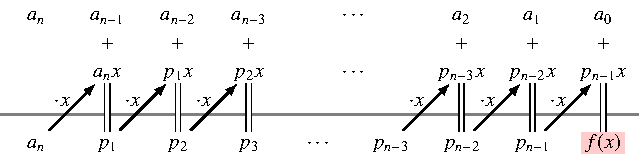
\includegraphics{chapters/20-gleichungen/figures/horner1.pdf}
\end{center}

\begin{beispiel}
Wir berechnen den Wert des Polyoms
\[
f(X) = X^6 - X^5 + X^4 - X^3 + X^2 - X + 1
\]
an der Stelle $X=2$ mit Hilfe des Horner-Schemas
\begin{center}
\begin{tabular}{>{$}r<{$}>{$}r<{$}>{$}r<{$}>{$}r<{$}>{$}r<{$}>{$}r<{$}>{$}r<{$}}
 1& -1& 1& -1&  1& -1&  1\\
  &  2& 2&  6& 10& 22& 42\\
\hline
 1&  1& 3&  5& 11& 21& 43
\end{tabular}
\end{center}
Der Wert in der rechten unteren Ecke stimmt überein mit
\begin{align*}
f(2)
&=
2^6-2^5+2^4-2^3+2^2-2+1
\\
&=
64-32+16-8+4-2+1
\\
&=
32+8+2+1
=
43.
\qedhere
\end{align*}
\end{beispiel}

\subsubsection{Deflation}
Die Bedeutung der Werte $p_0,\dots,p_{n-1}$ lässt sich verstehen, wenn
man den Polynomdivisionsalgorithmus für $f(X) / (X-x)$ ausschreibt.
\index{Polynomdivision}%
Die Rekursionsformeln~\eqref{buch:equation:reste} zeigen, dass die
Teilreste der Division die Koeffizienten $p_k$ haben:
\index{Division}%
\index{Teilreste}%
\begin{equation}
\setcounter{MaxMatrixCols}{20}
\setlength\arraycolsep{1pt}
\renewcommand\arraystretch{1.15}
\begin{matrix}
(a_nX^n&+&a_{n-1}X^{n-1}&+&a_{n-2}X^{n-2}&+&a_{n-3}X^{n-3}&+&\dots)&:&(X&-&x)&=&a_nX^{n-1}+p_1X^{n-2}+p_2X^{n-3}+\dots\\
 a_nX^n&-&a_{n}xX^{n-1} & &              & &              & &      & &  & &  & &                \\
\cline{1-3}
       & &p_1X^{n-1}    &+&a_{n-2}X^{n-2}& &              & &      & &  & &  & &                \\
       & &p_1X^{n-1}    &-&p_1xX^{n-2}   & &              & &      & &  & &  & &                \\
\cline{3-5}
       & &              & &p_2X^{n-2}    &+&a_{n-3}X^{n-3}& &      & &  & &  & &\\
       & &              & &p_2X^{n-2}    &-&a_{n-4}xX^{n-3}&&      & &  & &  &\\
\cline{5-7}
       & &              & &              & &p_3X^{n-3}     &&\dots & &  & &  &\\
       & &              & &              & &\dots          &&\dots & &  & &  &\\
\end{matrix}
\end{equation}
Die Koeffizienten $p_k$ sind daher auch die Koeffizienten des Quotienten
\[
q(X)
=
p_0X^{n-1}+p_1X^{n-2}+p_2X^{n-3}+\dots p_{n-2}X+p_{n-1}.
\]
Es gilt daher
\[
f(X)
=
(X-x) \cdot (p_0X^{n-1}+p_1X^{n-2}+p_2X^{n-3}+\dots p_{n-2}X+p_{n-1})
+
f(x).
\]
Ist $x$ ein Nullstelle, dann ist das Polynom ist $f(X)$ durch $X-x$ teilbar
und $q(X)$ ist der andere Faktor, also $f(X)=(X-x)\cdot q(X)$.
Das Polynom $q(X)$ hat Grad $n-1$, die Suche nach weiteren Nullstellen
wird also vereinfacht. 
Man nennt den Prozess, eine Nullstelle aus dem Polynom $f(X)$
herauszudividieren, {\em Deflation}.
\index{Nullstelle}%
\index{Deflation}%

\begin{beispiel}
Das Polynom
\[
f(x)=x^4-25x^2+144
\]
hat eine Nullstelle $x=3$ und $x=4$ als Nulllstellen.
Man finde zwei weitere Nullstellen.

Die Polynomdivision mit dem Horner-Schema für $x=3$
\begin{center}
\begin{tabular}{>{$}r<{$}>{$}r<{$}>{$}r<{$}>{$}r<{$}>{$}r<{$}}
   1&   0& -25&   0& 144\\
    &   3&   9& -48&-144\\
\hline
   1&   3& -16& -48&   0
\end{tabular}
\end{center}
ergibt 
\[
q_1(x) = f(x)/(x-3)
=
x^3+3x^2-16x-48
.
\]
Weiter bekommt man
\[
a_2(x) = f(x)/((x-3)(x-4)) = (x^2+7x+12) = (x+3)(x+4)
\]
aus
\begin{center}
\begin{tabular}{>{$}r<{$}>{$}r<{$}>{$}r<{$}>{$}r<{$}}
   1&   3& -16& -48\\
    &   4&  28&  48\\
\hline
   1&   7&  12&   0
\end{tabular}
\end{center}
Insbesondere schliesst man, dass $x=-3$ und $x=-4$ die verbleibenden
Nullstellen von $f(x)=(x-3)(x-4)(x+4)(x+3)$ sind.
\end{beispiel}


\subsubsection{Berechnung der Ableitung}
\index{Ableitung eines Polynoms}%
Für das Newton-Verfahren wird ausser dem Funktionswert auch die Ableitung
benötigt.
Der Funktionswert $r=f(x)$ wird mit dem Horner-Schema sofort gefunden, ebenso
\index{Horner-Schema}%
der Quotient $q(x)$,
Es gilt also
\[
f(X) = q(X)(X-x) + r,
\]
was wir dazu verwenden können, die Ableitung von $f$ mit Hilfe der
Produktregel zu berechnen:
\index{Produktregel}%
\[
f'(X) = q'(X) (X-x) + q(X).
\]
An der Stelle $X=x$ ist daher
$ f'(x) = q(x) $.
Da die Koeffizienten von $q(X)$ bereits mit dem Horner-Schema
berechnet worden sind, kann $f'(x)$ durch Iteration des Horner-Schemas
berechnet werden.

\begin{beispiel}
Man berechne den Funktionswert und die Ableitung des Polynoms
\[
f(x) = 2x^3 + x + 9
\]
an der Stelle $x=4$.
Zweimalige Anwendung des Horner-Schemas ergibt
\begin{center}
\begin{tabular}{>{$}r<{$}>{$}r<{$}>{$}r<{$}>{$}r<{$}}
   2&   0&   1&   9\\
    &   8&  32& 132\\
\hline
   2&   8&  33& 141\\
    &   8&  64&    \\
\hline
   2&  16&  97&
\end{tabular}
\end{center}
Man liest $f(4)=141$ und $f'(4)=97$ ab.
\end{beispiel}

Ist $x$ eine doppelte Nullstelle des Polynoms $f(x)$, dann ist $f'(x)=0$.
\index{Nullstelle!doppelte}%
\index{doppelte Nullstelle}%
Das Horner-Schema kann daher auch dazu verwendet werden, doppelte
Nullstellen zu erkennen und damit die Faktorisierung zu vereinfachen,
wie das folgende Beispiel zeigt.
\index{Faktorisierung}%

\begin{beispiel}
Wir betrachten das Polynom
\[
f(x) = x^4-13x^3 +41x^2 - 47x+18.
\]
Es hat die Nullstelle $x=1$, das Horner-Schema liefert für den Quotienten
\begin{center}
\begin{tabular}{>{$}r<{$}>{$}r<{$}>{$}r<{$}>{$}r<{$}>{$}r<{$}}
 1&-13& 41&-47& 18\\
  &  1&-12& 29&-18\\
\hline
 1&-12& 29&-18&  0\\
  &  1&-11& 18&   \\
\hline
 1&-11& 18&  0&   \\
  &  1&-10&   &   \\
\hline
 1&-10&  8&   &   
\end{tabular}
\end{center}
Daraus kann man ablesen, dass $x=1$ eine doppelte aber nicht
eine dreifache Nullstelle ist und dass sich das Polynom schreiben lässt als
\[
f(x)=(x-1)^2\cdot (x-11x+18) = (x-1)^2 (x-2)(x-9).
\]
Damit ist das Polynom $f(x)$ vollständig faktorisiert.
\end{beispiel}

\subsubsection{Newton-Verfahren für Nullstellen von Polynomen}
Da mit dem Horner-Schema sowohl Funktionswerte wie auch Ableitungen
effizient berechnet werden können, kann es dazu verwendet werden,
das Newton-Verfahren für Polynomnullstellen zu implementieren.

Das Horner-Schemas liefert zu jeder Nullstelle $x$ auch immer
gleich den Quotienten $q(X)=f(X)/(X-x)$, welches für die Suche nach
weiteren Nullstellen verwendet werden kann (Deflation).
\index{Deflation}%

\begin{beispiel}
\begin{table}
\centering
\renewcommand\arraystretch{1.15}
\begin{tabular}{|>{$}r<{$}|>{$}r<{$}|>{$}r<{$}|>{$}r<{$}|>{$}l<{$}|}
\hline
n& x_n & f(x_n) & f'(x_n) & q_n(X) \\
\hline
0&-10.000000& -182.00000&129.00000& X^2-X+19\\
1&- \underline{8}.589148&  -38.99232& 75.71571& X^2+0.4108524323 X+5.47112751\\
2& -\underline{8.0}74164&   -4.31028& 59.24143& X^2+0.9258356094 X+1.524651051\\
3& -\underline{8.00}1407&   -0.08021& 57.04221& X^2+0.9985933304 X+1.009848595\\
4& -\underline{8.000000}&   -0.00005& 57.00003& X^2+0.9999990463 X+1.000006676\\
5& -\underline{8.000000}&    0.00000& 57.00000& X^2+X+1\\
\hline
\end{tabular}
\caption{Newton-Verfahren für das Polynom $f(X)=X^3+9X^2+9X+8$
mit Hilfe des Horner-Schemas.
Als Nebeneffekt bestimmt das Horner-Schema in jeder Iteration auch
den Quotienten $q_n(x)=f(x)/(x-x_n)$.
\label{buch:table:hornernewton}}
\end{table}
Die reellen Nullstellen
von $f(X)=X^3+9X^2+9X +8$ sollen mit Hilfe des
Newton-Verfahrens gefunden werden.
Die Tabelle~\ref{buch:table:hornernewton} zeigt die vom Horner-Schema
berechneten Funktions- und Ableitungswerte sowie das Quotientenpolynom.
\index{Quotient!Polynom}%
Die Konvergenz ist quadratisch und liefert die Nullstelle $x=-8$
sowie den Quotienten $q(X)=X^2+X+1$,
tatsächlich ist
\[
(X+8)q(X) = (X+8)(X^2+X+1) = X^3+9X^2+9X+8 = f(X).
\]
Die Diskriminante von $q(X)$ ist
$b^2-4ac= 1^2 -4\cdot1\cdot 1= - 3<0$, $q(X)$ hat also keine weiteren
reellen Nullstellen.
\end{beispiel}

%
% normalverteilung.tex
%
% (c) 2020 Prof Dr Andreas Müller, Hochschule Rapeprswil
%
\subsection{Inverse der Normalverteilungsfunktion
\label{buch:subsection:inversenormal}}
Das Integral der Standardnormalverteilungsdichte
\[
\Phi(x) = \int_{-\infty}^x e^{-t^2/2}\,dt
\]
kann nicht in geschlossener Form berechnet werden und erst recht
nicht invertiert werden.
Für die Anwendung wird jedoch die Umkehrfunktion benötigt, zu einem Wert
$p\in[0,1]$ ist dasjenige $x$ zu finden, für welches $F(x)=p$ gilt.
Im Beispiel auf Seite~\pageref{buch:beispiel:erfc} wurde gezeigt,
wie die Fehlerfunktion
\[
\operatorname{erf}(x) = \frac{2}{\sqrt{\pi}}\int_0^x e^{-t^2}\,dt
\]
dazu verwendet werden kann
\[
\Phi(x) = \frac12+\operatorname{erf}(\sqrt{2}x)
\]
zu berechnen.
In diesem Abschnitt soll untersucht werden, wie zu gegebenen Funktionswert
das $x$ bestimmt werden kann.
Es soll also die Gleichung
\[
\Phi(x)=p
\qquad\Rightarrow\qquad
f(x)=\frac12+\operatorname{erf}(\sqrt{2}x)-p=0
\]
gelöst werden.

\subsubsection{Sekantenverfahren}
TODO

\subsubsection{Newton-Verfahren}
Das Newton-Verfahren benötigt ausser dem Funktionswert auch noch die 
Ableitung
\[
f'(x)
=
\frac{d}{dx}\frac{2}{\sqrt{\pi}}\int_0^{\sqrt{2}x} e^{-t^2}\,dt
=
\frac{2\sqrt{2}}{\sqrt{\pi}}e^{-2x^2}.
\]
Damit wird die Iterationsformel für das Newton-Verfahren:
\begin{equation}
x_{n+1} = x_n - \frac{\sqrt{\pi}}{2\sqrt{2}}e^{2x_n^2}
\biggl(\frac12+\operatorname{erf}(x_n) -p \biggr).
\end{equation}
Wie erwartet konvergiert die Iterationsfolge quadratisch für geeignete
Startwerte (siehe Tabelle~\ref{buch:table:normalnewton}).
Der Startwert $x_0=0$ funktioniert für jedes beliebige $p$.
Bei weiter von $0$ entfernten Starwerte läuft man Gefahr, dass die Iteration
zu betragsmässig grossen Werten $x$ springt, was dann zu einem Überlauf führt.

\begin{table}
\centering
\begin{tabular}{|>{$}r<{$}|>{$}r<{$}|}
\hline
 k &   x_n                    \\
\hline
 0 &   0.00000000000000000000 \\
 1 &   \underline{0.2}5066282746310003808 \\
 2 &   \underline{0.262}13276541328668328 \\
 3 &   \underline{0.26220025}396582809170 \\
 4 &   \underline{0.2622002563540203}8710 \\
 5 &   \underline{0.262200256354020390}13 \\
 6 &   \underline{0.262200256354020390}05 \\
 7 &   \underline{0.262200256354020390}13 \\
 8 &   \underline{0.262200256354020390}05 \\
 9 &   \underline{0.262200256354020390}13 \\
\hline
\end{tabular}
\caption{Newton-Iteration zur Bestimmung der Inversen der Verteilungsfunktion
der Normalverteilung, berechnet mit dem Typ \texttt{long double}.
Die letzten zwei Stellen können wegen numerischer Unsicherheit nicht
berechnet werden.
\label{buch:table:normalnewton}}
\end{table}








